\documentclass[12pt,a4paper]{report}
\usepackage[utf8]{inputenc}
\usepackage[T1]{fontenc}
\usepackage[english,italian]{babel}
\usepackage{amsmath}
\usepackage{amssymb}
\usepackage{amsfonts}
\usepackage{mathrsfs}
\usepackage{graphicx}
\usepackage{amsthm}
\usepackage{newlfont}
\usepackage{color}
\usepackage{natbib}
\usepackage{float}
\usepackage{textcomp}

\textwidth=450pt\oddsidemargin=0pt

\begin{document}

\begin{titlepage}

%
%
% UNA VOLTA FATTE LE DOVUTE MODIFICHE SOSTITUIRE "RED" CON "BLACK" NEI COMANDI \textcolor
%
%
\begin{center}
{{\Large{\textsc{Alma Mater Studiorum $\cdot$ Universit\`a di Bologna}}}} 
\rule[0.1cm]{15.8cm}{0.1mm}
\rule[0.5cm]{15.8cm}{0.6mm}
\\\vspace{3mm}

{\small{\bf Scuola di Scienze \\ 
Dipartimento di Fisica e Astronomia\\
Corso di Laurea in Fisica}}

\end{center}

\vspace{23mm}

\begin{center}\textcolor{red}{
%
% INSERIRE IL TITOLO DELLA TESI
%
{\LARGE{\bf TITOLO TESI}}\\
}\end{center}

\vspace{50mm} \par \noindent

\begin{minipage}[t]{0.47\textwidth}
%
% INSERIRE IL NOME DEL RELATORE CON IL RELATIVO TITOLO DI DOTTORE O PROFESSORE
%
{\large{\bf Relatore: \vspace{2mm}\\\textcolor{red}{
Prof./Dott. Enrico Giampieri}\\\\
%
% INSERIRE IL NOME DEL CORRELATORE CON IL RELATIVO TITOLO DI DOTTORE O PROFESSORE
%
% SE NON AVETE UN CORRELATORE CANCELLATE LE PROSSIME 3 RIGHE
%
\textcolor{red}{
\bf Correlatore: (eventuale)
\vspace{2mm}\\
Prof./Dott. Nome Cognome\\\\}}}
\end{minipage}
%
\hfill
%
\begin{minipage}[t]{0.47\textwidth}\raggedleft \textcolor{black}{
{\large{\bf Presentata da:
\vspace{2mm}\\
%
% INSERIRE IL NOME DEL CANDIDATO
%
Mattia Ceccarelli}}}
\end{minipage}

\vspace{40mm}

\begin{center}
%
% INSERIRE L'ANNO ACCADEMICO
%
Anno Accademico \textcolor{black}{ 2017/2018}
\end{center}

\end{titlepage}

%\thispagestyle{empty}
%\clearpage\null\newpage

\tableofcontents
%\clearpage{\pagestyle{empty}\cleardoublepage}1


\chapter{Introduzione}

In questo capitolo si introdurranno i principali mezzi utilizzati nello svolgimento del progetto di tesi, ossia Algoritmi Genetici per la ricerca dei minimi di una funzione non parametrica \underline{?????} e Reti Neurali \textit{fully connected}, che svolgono il ruolo di funzione a molti parametri da ottimizare in un problema di classificazione.

\section{Algoritmi Genetici}\label{alg-gen}

Gli algoritmi genetici sono software di ricerca ispirati dalla selezione naturale applicata ad una popolazione di individui, chiamati soluzioni, caratterizzati da un \textit{cromosoma}, spesso rappresentato da una lista di numeri binari o da una  stringa.
Il parametro che differenzia soluzioni migliori o peggiori è il \textit{fitness}, misurato attraverso la \textit{funzione di fitness} la quale dipende dal problema.
L' evoluzione della popolazione avviene attraverso la selezione dei migliori individui che passeranno il loro \textit{cromosoma} alla generazione successiva.

\subsection{Operatori}

\cite{genetic-algorithm-mitchell}
I principali operatori che compongo un semplice algoritmo genetico sono:

\paragraph{Selezione} Questo operatore seleziona i migliori individui, più è alto è il fitness e più è probabile che un individuo venga scelto per creare la nuova generazione

\paragraph{Crossover} L'operatore di Crossover produce un taglio nel genoma degli individui ``genitori`` per formare due individui ''figli'': per esempio prendendo le due stringhe 111000 e 000111, producendo un taglio alla terza posizione otterremo le stringhe  111111 e 000000.

\paragraph{Mutazione} L'operatore di mutazione si occupa di cambiare casualmente uno o più caratteri di individui scelti a caso nella popolazione.

Il funzionamento di un tipico algoritmo genetico,come descritto da \cite{genetic-algorithm-mitchell} una volta definito il problema,  procede in questo modo:

\subsection{Struttura di un Algoritmo Genetico}

\begin{enumerate}
 \item Creazione casuale di \textit{n} elementi, che rappresentano la prima popolazione. 
 \item Calcolo del fitness $f(x)$ di ogni soluzione $x$ della popolazione.
 \item Fino a che non sono stati generati \textit{n} discendenti ripetere:
 \begin{enumerate}
  \item[a.] Selezione di due genitori dalla popolazione dove un individuo può anche essere scelto più volte.
  \item[b.] Con probabilità $p_{c}$ (probabilità di crossover) applicare l'operatore di crossover sui due genitori. Nel caso non avvenisse alcun crossover, copiare i genitori.
  \item[c.] Con probabilità $p_{m}$ (probabilità di mutazione) applicare l'operatore di mutazione sui figli.
 \end{enumerate}
 \item Sostituire la vecchia popolazione con la nuova generazione e ripetere dal secondo passaggio.
\end{enumerate}

Ogni iterazione di questo processo è chiamata \textit{generazione}.

\subsection{Applicazioni}

Il classico esempio di utilizzo di un algoritmo genetico è la ricerca dei massimi di una funzione.
In tal caso, un individuo è rappresentato da una stringa di bit, la \textit{funzione di fitness} è la funzione stessa e il \textit{fitness} delle soluzioni è il valore della funzione calcolato nel punto di cui l'individuo è la rappresentazione binaria.
Oltre ad essere l'esempio più semplice risulta anche quello più significativo: di fatto lo scopo di un algoritmo genetico è ottimizzare.
\\
Da migliorare

\section{Reti Neurali}

Una rete neurale è una struttura interconnessa di semplici unità procedurali, chiamate nodi. La loro funzionalità si ispira ai neuroni del regno animale. La capacità di elaborazione della rete neurale è contenuta nella ``forza`` delle connessioni tra nodi, espressa dai \textit{pesi} dei collegamenti, ottenuti da processi di \textit{ addestramento} o \textit{apprendimento}. \cite{neural-net-gurney}

\subsection{Perceptron}

\cite{neural-net-nielsen}
Il perceptron è stato sviluppato negli anni '50 e '60 dal ricercatore Frank Rosenblatt ispirandosi ai lavori antecedenti di Warren McCulloch e Walter Pitts.
È l'unità di base di una rete neurale e il suo funzionamento è il seguente:
il perceptron riceve $n$ valori in ingresso $x_{1},x_{2},...,x_{n}$ e restituisce $1$ o $0$ a seconda che la somma pesata degli input superi o no un valore di soglia, con pesi $w_{1},w_{2},...,w_{n}$.
Ad esempio nel perceptron mostrato in figura \ref{perceptron}:

\begin{figure}[H]
 \centering
 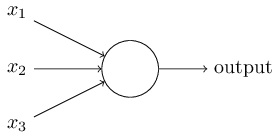
\includegraphics[scale = 0.7]{images/perceptron.png}
 \caption{\textit{Perceptron con 3 input ed un output}}
 \label{perceptron}
\end{figure}

l'output sarà determinato da:

\begin{center}
$\begin{cases}
 0 \text{ se } \sum_{i} x_{i}w_{i} \leq valore\text{ }di\text{ }soglia\\
 1 \text{ se } \sum_{i} x_{i}w_{i} > valore\text{ }di\text{ }soglia 
\end{cases} $
\end{center}

anche se è più comune trovare la scrittura:

\begin{center}
$\begin{cases}
 0 \text{ se } \sum_{i} x_{i}w_{i} + b \leq 0\\
 1 \text{ se } \sum_{i} x_{i}w_{i} + b > 0
\end{cases}$
\end{center}

dove $b$ è detto \textit{bias} del perceptron.
È attraverso \textit{pesi} e \textit{bias} che il perceptron può soppesare diverse prove e compiere decisioni.

Tuttavia se la rete contenesse perceptron, anche un piccolo cambiamento nei parametri interni potrebbe causare un cambiamento netto nel comportamento della rete [\cite{neural-net-nielsen}], per questo è preferibile utilizzare una \textit{funzione di attivazione} che rende continuo l'output di un nodo.
Un esempio di funzione di attivazione è la sigmoide definita come:

\begin{equation} \label{sigma}
 \sigma(z) = \frac{1}{1+e^{-z}} 
\end{equation}

e l'output di un nodo della rete diventa :

\begin{equation} \label{z}
  y = \sigma(\sum_{i}{x_{i}w_{i}} + b)
\end{equation}

risultato che è continuo e compreso tra zero ed uno.

Un altro tipo di funzione di attivazione è la \textit{Rectified Linear Units} o \textit{ReLU} e si presenta come:

\begin{equation}
 y(x) = max \{0,x\} 
\end{equation}

\begin{figure}[H]
 \centering
 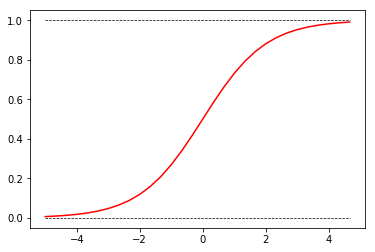
\includegraphics[scale = 0.5]{images/sigmoide.png}
 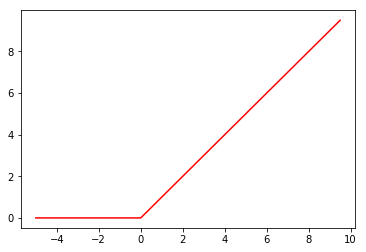
\includegraphics[scale = 0.5]{images/relu.png}
 \caption{\textit{confronto tra due funzioni di attivazione: a sinistra sigmoidale e a destra ReLU}}
 \label{sigmarelu}
\end{figure}

La scelta della migliore funzione di attivazione non è univoca e dipende dal problema che viene affrontato.

\subsection{Struttura \textit{fully connected}}

La struttura di una rete neurale \textit{fully connected} composta da molti \textit{layer} di neuroni è come quella mostrata in figura \ref{net}:

\begin{figure}[H]
 \centering
 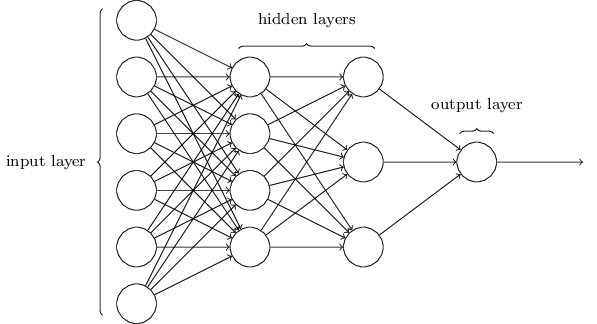
\includegraphics[scale = 0.5]{images/net.png}
 \caption{\textit{Esempio di rete neurale fully connected in cui viene mostrata la distinzione tra input layer, hidden layer e output layer}}
 \label{net}
\end{figure} 

In una rete come questa ad ogni collegamento è associato un peso e ad ogni nodo è associato un \textit{bias}: gli output dei \textit{neuroni} del \textit{layer} di input diventano a loro volta valori in ingresso del \textit{layer} successivo in un procedimento a catena fino all'ultimo \textit{layer}, che restituisce la risposta della rete. 
L'addestramento della rete consiste nel valutarne gli output in un determinato set di dati, chiamato \textit{training dataset}, confrontarli con i valori attesi, forniti dallo stesso \textit{dataset}, e modificare pesi e \textit{bias} in modo che la risposta si avvicini a ciò che ci si aspetta.


Da completare con accenno a BackPropagation

\subsection{Evoluzione di una Rete Neurale}

\chapter{Metodologia}

In questo capitolo verranno descritti i metodi utilizzati per l'ottimizzazione di una rete neurale \textit{fully connected} attraverso un algoritmo genetico: l' obiettivo è quello di evolvere la struttura degli \textit{hidden layer} della rete al fine di classificare al meglio 
un dataset separato in due classi di dati.

\section{Popolazione di reti neurali}

L'algoritmo genera la prima popolazione di oggetti \textit{Random Network} casualmente, i parametri interni sono stati scelti in modo che questa fosse limitata e non raggiungesse subito un risultato ottimale.
In particolare il numero di layer è compreso tra 1 e 5 mentre il numero massimo di neuroni per layer è 25.
La popolazione è stata mantenuta al massimo di 20 individui per lo stesso motivo.
Il \textit{cromosoma} di un individuo è quindi una lista di numeri di lunghezza variabile e l'algoritmo genetico è stato adattato a questo problema: la ricerca di un minimo in uno spazio in cui il numero di variabili non è definito.

\section{Operatori}

La differenza nell'utilizzare cromosomi di lunghezza variabile si ritrova soprattutto negli operatori dell'algoritmo genetico scritto \textit{ad hoc} per il progetto che devono gestire una variabile che normalmente non rappresenterebbe un problema. 
Per questo ogni operatore è stato adattato per fare in modo che sia possibile esplorare lo spazio delle soluzioni anche in tal senso.

\subsection{Crossover}

Il Crossover si differenzia da quello di un algoritmo genetico in cui la lunghezza di ogni cromosoma sia prestabilita. 
Infatti, è facile che i due genitori selezionati non abbiano lo stesso numero di hidden layer: in questo caso non è possibile ''tagliare'' il cromosoma nello stesso punto (come mostrato nel capitolo \ref{alg-gen}).
Inoltre è necessario che la lunghezza dei figli possa essere diversa da quella dei genitori in modo da non limitare le possibilità di esplorazione.

Seguendo questi propositi, vengono scelti casualmente due punti di taglio, uno per genitore, da una media di tre interi casuali (questo per fare in modo che la lunghezza non cambi troppo tra una generazione e la successiva).
Dopodiché il crossover procede come in un classico algoritmo genetico, ossia restituendo due figli combinazione delle parti tagliate.

Un esempio di funzionamento, scelti i genitori:

\begin{center}
 genitore 1 = [10,3,4,11];  genitore 2 = [7,23,1,2,19]\\
\end{center}

e prendendo due tagli rispettivamente alla $3^{a}$ e $2^{a}$ posizione si ottengono:

\begin{center}
 figlio 1 = [10,3,4,1,2,19]; figlio 2 = [7,23,11]
\end{center}

i quali popoleranno la generazione successiva.

\subsection{Mutazione}

Anche il processo di mutazione ha subito qualche variazione, infatti, occorre che anche la lunghezza del cromosoma possa cambiare a seguito dell'azione di questo operatore.
Per fare ciò sono state introdotte due probabilità indipendenti: $p_{m} = 5$\textdiscount \text{ }rappresenta la probabilità che un layer qualsiasi del cromosoma venga modificato aggiungendo o togliendo un neurone, $p_{l} = 5$\textdiscount \text{ }rappresenta invece la probabilità che venga aggiunto o rimosso un layer dalla rete.

\subsection{Selezione}

Nella varietà di operatori di selezione, verranno comparati i risultati di due algoritmi, scelti per la semplicità di implementazione che nulla toglie alla capacità di questi di evolvere il sistema.

\begin{enumerate}
 \item Il primo, denominato \textit{random mate}, è il più rapido: partendo da una popolazione ordinata per miglior \textit{fitness} passa alla nuova generazione un' \textit{élite} di individui pari al 20\textdiscount.
 Poi scorre dall'inizio la popolazione per il primo genitore, mentre il secondo genitore viene scelto a caso. 
 Questo avviene fino a che la generazione successiva non è riempita.
 
 \item Il secondo, denominato \textit{all sons}, è concettualmente più semplice ma richiede molto più tempo per completare una run: continuando a mantenere un 20\textdiscount di \textit{élite}, in una popolazione viene fatto il crossover di ogni coppia possibile di individui.
 Di questi vengono scelti i migliori per riempire la generazione successiva.
 È facile capire come questo sia il metodo più dispendioso in termini di risorse, infatti ogni rete va addestrata per determinarne il \textit{fitness} e in una popolazioni di soli 10 individui il numero totale di reti da valutare per ogni generazione sale a 200 =  ($10*10*2$)
 
\end{enumerate}

Mantenere un'\textit{élite} di individui è utile per fare in modo che la popolazione evolva ma allo stesso tempo mantenga intatti i caratteri che nella precedente generazione hanno conseguito il miglior score.

\section{Funzione di Fitness}

La funzione di fitness dell'algoritmo riceve il cromosoma di ogni individuo che come mostrato in sezioni precedenti ha la forma di una lista di interi, che rappresentano gli \textit{hidden layer} della rete.
È a questo punto che viene costruita la rete vera e propria, che altro non è che un'istanza della classe \textit{MLPClassifier} (che sta per \textit{Multi-layer Perceptron classifier}) della libreria \textit{scikit learn} (\cite{scikit-learn}).

L'addestramento della rete è affidato alla funzione \textit{fit}, propria di ogni Classificatore di \textit{scikit learn}, che restituisce un oggetto \textit{MLP} addestrato sul \textit{training set}.

A questo punto è possibile misurare la risposta di un \textit{MLP} addestrato agli input: l'\textit{input layer} è composto da due nodi, ossia le due coordinate di un punto, l'\textit{output layer} da un solo nodo, con output compreso tra 0 (classe 1) e 1(classe 2) come mostrato in figura \ref{MLP}:

\begin{figure}[H]
 \centering
 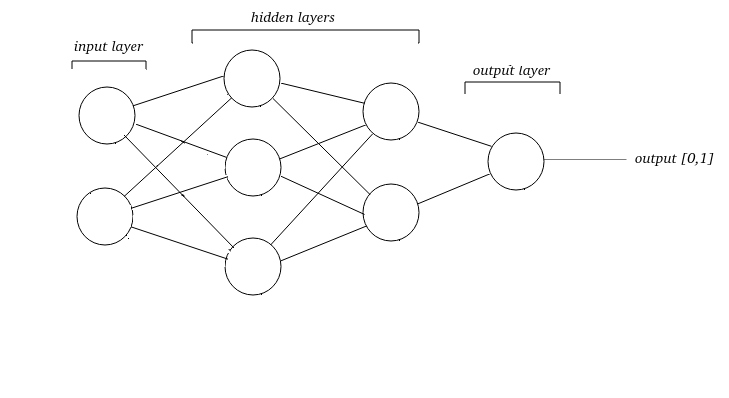
\includegraphics[scale = 0.55]{images/MLPClass}
 \caption {\textit{Esempio di MLPClassier generato da un individuo con cromosoma [3,2]}}
 \label{MLP}
\end{figure}

Infine si sfrutta il \textit{test set} per attribuire un \textit{fitness}, o \textit{score}, all'individuo.
Ciò viene fatto utilizzando due metri di valutazione differenti, valutati in parallelo: 

\paragraph{\textit{Accuracy score}} questo metodo è il più semplice e diretto: attribuisce un fitness pari alla percentuale di risposte corrette della rete. Il problema di questo procedimento è che equipara una risposta di $0.51$ ad $1$ ed una di $0.49$ a $0$ nonostante in entrambe le risposte l'incertezza sia alta.
L'\textit{accuracy score} viene massimizzato nell'algoritmo.

\paragraph{\textit{Logarithmic loss function}} o \textit{log loss}, è una misura di quanta incertezza pone la rete nelle sue risposte. Dalla documentazione di \textit{scikit learn} la \textit{log loss} è definita come "\textit{the negative log-likehood of the true labels given a probabilistic classifier's prediction}" o :  

\begin{equation}
 -log P(\frac{y_{t}}{y_{p}}) = -(y_{t} log(y_{p}) + (1 - y_{t}) log(1 - y_{p}))
\end{equation}
Dove $y_{t}$ è la classe dell'oggetto (o $0$ o $1$ ), mentre $y_{p}$ è la probabilità stimata che l'oggetto sia di quella classe.

\section{Datasets}

I set di dati sono artificiali e forniti da \textit{scikit learn}. 
Sono stati usati per le prove 3 tipi di dataset:

\paragraph{moons} I punti rossi e blu vengono generati a forma di semicerchi, come mostrato in figura \ref{moons} 

\begin{figure}[H]
 \centering
 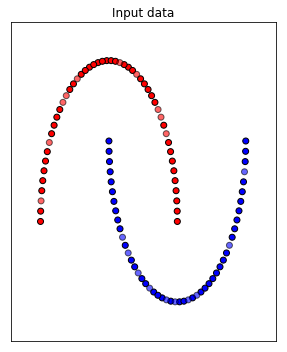
\includegraphics[scale = 0.5]{images/moons_nonoise}
 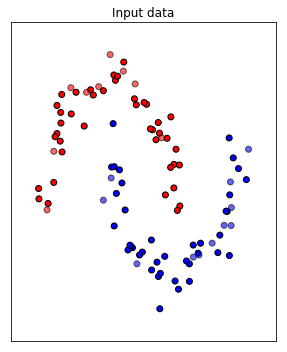
\includegraphics[scale = 0.5]{images/moons_noise}
 \caption{\textit{Nell'immagine sono messe a confronto due versioni del dataset moons: a sinistra priva di noise e a destra con noise = 0.1}}
 \label{moons}
\end{figure}

\paragraph{circles} I punti vengono generati a forma di cerchi concentrici, è possibile fornire diversi gradi di separazione ai due cerchi attraverso il parametro \textit{factor}. Il dataset è mostrato in figura \ref{circles}

\begin{figure}[H]
 \centering
 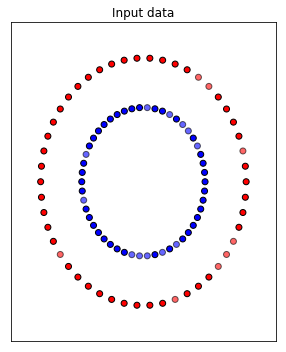
\includegraphics[scale = 0.5]{images/circles_nonoise}
 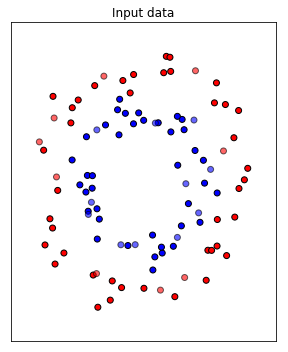
\includegraphics[scale = 0.5]{images/circles_noise}
 \caption{\textit{Nell'immagine a confronto due versioni del dataset circles: a sinistra senza noise e a destra con noise = 0.1. Entrambe con lo stesso fattore tra i cerchi}}
 \label{circles}
\end{figure}

\paragraph{circles+} È un dataset personalizzato creato dall'unione di due "circles", come mostrato in figura \ref{circles+}

\begin{figure}[H]
 \centering
 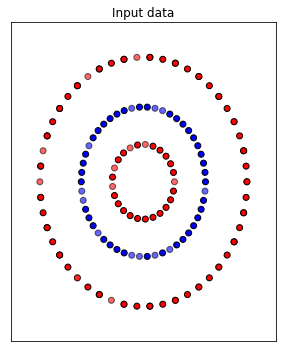
\includegraphics[scale = 0.5]{images/circles+_nonoise}
 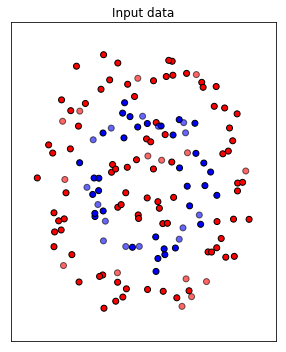
\includegraphics[scale = 0.5]{images/circles+_noise}
 \caption{\textit {Nell'immagine a confronto due versioni del dataset circles+: a sinistra con noise = 0 e a destra con noise = 0.1 }}
 \label{circles+}
\end{figure}

Per tutti i datasets è possibile attribuire un \textit{noise} in modo che sia più difficile classificarli.
Nel corso delle prove sono state valutate le prestazioni dell'algoritmo su tutti i datasets.
Sono stati appositamente evitati dataset lineramente separabili.

I dataset sono generati a partire dalle due funzioni \textit{make moons} e \textit{make circles} di \textit{scikit learn}.

%FORSE QUALCOSA SU TRAIN_TEST_SPLIT e TRASFORMATION

\section{Struttura dell'algoritmo }

Per chiarezza viene riportata la struttura dell'algoritmo, che ne mostra i vari passaggi:

\begin{enumerate}
 \item creazione della prima generazione.
 \item generazione del dataset, separazione di questo in \textit{train set} e \textit{test set}, valutazione del \textit{fitness} e ordinamento della popolazione.
 \item finché l'individuo con il \textit{best fitness} non rimane lo stesso per 5 generazioni consecutive:
 \begin{enumerate}
  \item[a.] separazione del dataset in \textit{train set} e \textit{test set} con \textit{random state} differenti ad ogni ciclo.
  \item[b.] Finchè la nuova generazione non è riempita ripetere:
  \begin{enumerate}
   \item [-] Selezione del primo e secondo genitore.
   \item [-] Crossover e creazione dei figli.
   \item [-] Mutazione dei figli.
  \end{enumerate}
  \item [c.] Valutazione del fitness e ordinamento della nuova generazione
  \item [d.] Risulatati del migliore individuo sul dataset scelto.
 \end{enumerate}
 \item Termine algoritmo.
\end{enumerate}


\chapter{Risultati}

\chapter{Conclusioni}

\listoffigures

\nocite{*}
\addcontentsline{toc}{chapter}{Bibliografia}
\bibliographystyle{plainnat}
\bibliography{Bibliografia.bib}


\end{document}




